 


% In this thesis, we make contributions at the intersection between neural networks and structured matrices.
We build neural networks with structured matrices and develop new methods for training neural networks whose efficiency relies on the properties of structured matrices. 
% on certain properties of structured matrices.
Hereafter, we present the preliminary knowledge on the theory of structured matrices that is required for the contribution of this thesis. 


%%%%%%%%%%%%%%%%%%%%%%%%%%%%%%%%%%%%%%%%%%%%%%%%%%%%%%%%%%%%%%%%%%%%%%%%%%%%%%%
\subsection{Properties of Circulant Matrices}
\label{subsection:ch2-properties_of_circulant_matrices}
%%%%%%%%%%%%%%%%%%%%%%%%%%%%%%%%%%%%%%%%%%%%%%%%%%%%%%%%%%%%%%%%%%%%%%%%%%%%%%%

A circulant matrix is a matrix in which each descending diagonal, from left to right, is constant and each row of the matrix is a cyclic right shift of the previous one:
\begin{equation}
  \Cmat =
  \leftmatrix
    c_0 & c_{n-1} & c_{n-2} & \cdots & \cdots & c_{1} \\
    c_{1} & c_0 & c_{n-1} & \ddots & & \vdots \\
    c_{2} & c_{1} & \ddots & \ddots & \ddots & \vdots \\
    \vdots & \ddots & \ddots & \ddots & c_{n-1} & c_{n-2} \\
    \vdots & & \ddots & c_{1} & c_{0} & c_{n-1} \\
    c_{n-1} & \cdots & \cdots & c_{2} & c_{1} & c_0
  \rightmatrix
\end{equation}
\noindent
The $n \times n$ circulant matrix $\Cmat$ is fully determined by the sequence of scalars $\{c_h\}_{h \in \Iset^+_n}$ where $\Iset^+_n= \{0, \ldots, n-1\}$.
Furthermore, the $(j,k)$ entry of $\Cmat$ is given by
\begin{equation}
  \leftmat \Cmat \rightmat_{j,k} = c_{\left(k-j\right) \mod n} \enspace.
\end{equation}

% For the contributions of this thesis, we will use the properties of circulant matrices, specifically their compact representation and their ability to accelerate the matrix-vector product operation.
% These properties are due to their special eigenvectors and a closed formula on their eigenvalues as we will see in the following.


\begin{algorithm}[htb]
  \begin{algorithmic}[1]
    \Procedure{CIRCMUL}{$\cvec, \xvec$} \Comment{first column of the circulant matrix $\Cmat$, vector $\xvec$}
      \State $\tilde{\xvec} \gets \textbf{FFT}(\xvec)$
      \State $\tilde{\cvec} \gets \textbf{FFT}(\cvec)$
      \State $\yvec \gets \textbf{IFFT}(\tilde{\xvec} \odot \tilde{\cvec})$ \Comment{element-wise vector-vector product}
      \State \textbf{return} $\yvec$ \Comment{return the result of the product $\Cmat \xvec$}
    \EndProcedure
  \end{algorithmic}
  \caption{Matrix-vector product with a circulant matrix}
  \label{algorithm:ch2-matrix_vector_product_circulant_matrix}
\end{algorithm}

In numerical analysis, circulant matrices are important due to their numerous properties.
Indeed, circulant matrices can be compactly represented in memory using only $n$ values instead of $n^2$ values required for arbitrary matrices.
In addition, algorithms exist to accelerate the matrix-vector product operation from $\bigO(n^2)$ to $\bigO(n \log n)$. 
Finally, circulant matrices commute and are closed under the sum and products.
All these properties can be demonstrated with the special diagonalization of circulant matrices with the matrix expansion of the Discrete Fourier Transform (DFT), \ie, Fourier matrix, and an explicit formula of their eigenvalues.
The Fourier matrix is of the form:
\begin{definition}[Fourier Matrix]
  The Fourier matrix of order $n$ is defined as follows:
  \begin{equation} \label{definition:ch2-fourier_matrix}
    \Umat_n = 
    \leftmatrix
      1      & 1         & 1            & \cdots & 1                \\
      1      & z_n       & z_n^2        & \cdots & z_n^{n-1}        \\
      1      & z_n^2     & z_n^4        & \cdots & z_n^{2(n-1)}     \\
      \vdots & \vdots    & \vdots       &        & \vdots           \\
      1      & z_n^{n-1} & z_n^{2(n-1)} & \cdots & z_n^{(n-1)(n-1)}
    \rightmatrix
  \end{equation}
  where $z_n = e^{-\frac{2\pi\ci}{n}}$ is an $n^{\text{th}}$ root of unity.
\end{definition}
\noindent
The diagonalization of circulant matrices is presented in the following theorem:
\begin{theorem}[Theorem 3.1 of \citet{gray2006toeplitz}] \label{theorem:ch2-diagonalization_circulant_matrix}
  The eigenvalues $\lambda_k$ and the eigenvectors $\yvec^{(k)}$ of a circulant matrix $\Cmat = \circulant(\cvec)$ with $\cvec \in \Rbb^n$ are as follows:
  \begin{equation}
    \lambda_k = \sum_{j \in \Iset^+_n} c_j e^{-\frac{2 \pi \ci}{n} jk} \quad \Leftrightarrow \quad \psi_k = \left( \Umat \cvec \right)_k
  \end{equation}
  and
  \begin{equation}
    \yvec^{(k)} = \frac{1}{\sqrt{n}} \leftmatrix 1, e^{-\frac{2 \pi \ci k}{n}}, \dots, e^{-\frac{2 \pi \ci k(n-1)}{n}} \rightmatrix^\top
  \end{equation}
  Furthermore, the circulant matrix $\Cmat$ can be expressed in the form 
  \begin{equation} \label{equation:ch2-diagonalization_circulant_matrix}
    \Cmat = \frac{1}{n} \Umat_n^* \diag(\Umat_n \cvec) \Umat_n \enspace.
  \end{equation}
\end{theorem}


\begingroup
\allowdisplaybreaks

\noindent
Based on this decomposition, we can recover several important properties of circulant matrices:
\begin{itemize}[leftmargin=13pt]
  \item \textbf{Matrix-vector product}: Let $\xvec \in \Rbb^n$ an arbitrary vector then the product $\Cmat \xvec$ can be expanded as follows:
  \begin{align}
    \Cmat \xvec &= \frac{1}{n} \Umat_n^* \diag(\Umat_n \cvec) \Umat_n \xvec  \\
    &= \frac{1}{n} \Umat_n^* \left( \big(\Umat_n \cvec \big) \odot \big( \Umat_n \xvec \big) \right)
  \end{align}
  Thus, the matrix-vector product $\Cmat \xvec$ can be reduced to an element-wise multiplication between the characteristic vector $\cvec$ and the vector $\xvec$ in the Fourier domain.
  Furthermore, the multiplication between the Fourier matrix $\Umat_n$ and a vector can be efficiently computed with the \emph{Fast Fourier Transform} (FFT) algorithms~\cite{cooley1965algorithm}.
  \Cref{algorithm:ch2-matrix_vector_product_circulant_matrix} details the steps required to perform the $\bigO(n \log n)$ multiplication between  a circulant matrix and a vector.
\item \textbf{Closeness under sum}: Let $\xvec, \yvec \in \Rbb^n$, let $\Xmat= \circulant(\xvec)$ and $\Ymat = \circulant(\yvec)$ then, $\Zmat  = \Xmat + \Ymat$ is also a circulant matrix with $\Zmat = \circulant(\xvec + \yvec)$:
    \begin{align}
      \Xmat + \Ymat &= \left( \frac{1}{n} \Umat_n^* \diag(\Umat_n \xvec) \Umat_n \right) + \left( \frac{1}{n} \Umat_n^* \diag(\Umat_n \yvec) \Umat_n \right) \\
      &= \frac{1}{n}  \Umat_n^* \left( \diag(\Umat_n \xvec) \Umat_n  + \diag(\Umat_n \yvec) \Umat_n \right) \\
      &= \frac{1}{n}  \Umat_n^* \left( \diag(\Umat_n \xvec) + \diag(\Umat_n \yvec) \right) \Umat_n  \\
      &= \frac{1}{n}  \Umat_n^* \left( \diag(\Umat_n (\xvec + \yvec)) \right) \Umat_n  \\
      &= \circulant(\xvec + \yvec)
    \end{align}
  \item \textbf{Closeness under product}: Let $\xvec, \yvec \in \Rbb^n$, let $\Xmat= \circulant(\xvec)$ and $\Ymat = \circulant(\yvec)$ then, $\Zmat  = \Xmat \Ymat$ is also a circulant matrix with $\Zmat = \circulant(\xvec \odot \yvec)$:
    \begin{align}
      \Xmat \Ymat &= \left( \frac{1}{n} \Umat_n^* \diag(\Umat_n \xvec) \Umat_n \right) \left( \frac{1}{n} \Umat_n^* \diag(\Umat_n \yvec) \Umat_n \right) \\
      &= \frac{1}{n^2}  \Umat_n^* \diag(\Umat_n \xvec) \Umat_n \Umat_n^* \diag(\Umat_n \yvec) \Umat_n  \\
      &= \frac{1}{n^2}  \Umat_n^* \diag(\Umat_n \xvec) (n \Imat) \diag(\Umat_n \yvec) \Umat_n  \\
      &= \frac{1}{n}  \Umat_n^* \diag(\Umat_n \xvec) \diag(\Umat_n \yvec) \Umat_n  \\
      &= \frac{1}{n}  \Umat_n^* \diag(\Umat_n (\xvec \odot \yvec)) \Umat_n  \\
      &= \circulant(\xvec \odot \yvec)
    \end{align}
\end{itemize}

\endgroup



In this thesis, we also make use of specific type of circulant matrices called \emph{$f$-circulant matrices} which are one of the building blocks of \emph{low displacement rank operators} presented in \Cref{subsection:ch2-general_frameworks_for_structured_matrices} and also enjoy compact representation and fast matrix-vector product.
A $f$-unit-circulant matrix is defined as follows:
\begin{definition}[$f$-circulant matrix] \label{definition:ch2-f_circulant_matrix}
  Given a vector $\xvec$ and a scalar $f$, the $f$-circulant matrix, $\Zmat_f(\xvec)$, is defined as follows:
  \begin{equation}
    \Zmat_f(\xvec) \triangleq
    \leftmatrix
      \xvec_0 & $f$ \xvec_{n-1} & $f$ \xvec_{n-2} & \cdots & \cdots & $f$ \xvec_{1} \\
      \xvec_{1} & \xvec_0 & $f$ \xvec_{n-1} & \ddots & & \vdots \\
      \xvec_{2} & \xvec_{1} & \ddots & \ddots & \ddots & \vdots \\ 
      \vdots & \ddots & \ddots & \ddots & $f$ \xvec_{n-1} & $f$ \xvec_{n-2} \\
      \vdots & & \ddots & \xvec_{1} & \xvec_{0} & $f$ \xvec_{n-1} \\
      \xvec_{n-1} & \cdots & \cdots & \xvec_{2} & \xvec_{1} & \xvec_0
    \rightmatrix
  \end{equation}
  \removespace
\end{definition}
\noindent
We denote $\Zmat_f$ the $f$-unit-circulant, defined by the vector $\left(0, 1, \dots, 0 \right)^\top$, a matrix of the form:
% \begin{equation}
%   \Zmat_f = \circulant \big(e^{(1)} \big) + (f - 1) \evec^{(0)} \evec^{(n-1)\top}
% \end{equation}
% \noindent
\begin{equation}
  \Zmat_f = 
    \leftmatrix
      0      & 0      & 0      & \cdots & \cdots & f      \\
      1      & 0      & 0      & \ddots &        & \vdots \\
      0      & 1      & \ddots & \ddots & \ddots & \vdots \\ 
      \vdots & \ddots & \ddots & \ddots & 0      & 0      \\
      \vdots &        & \ddots & 1      & 0      & 0      \\
      0      & \cdots & \cdots & 0      & 1      & 0
    \rightmatrix
\end{equation}
\noindent
The matrix-vector product $\Zmat_f \xvec$ scales the last element by $f$ and makes a circular shift on the components of the vector $\xvec$ by one resulting in $\Zmat_f \xvec = \leftmat f \xvec_{n-1}, \xvec_0, \dots, \xvec_{n-2} \rightmat^\top$.


%%%%%%%%%%%%%%%%%%%%%%%%%%%%%%%%%%%%%%%%%%%%%%%%%%%%%%%%%%%%%%%%%%%%%%%%%%%%%%%%
\subsection{A Fourier Representation of Toeplitz Matrices}
\label{subsection:ch2-a_fourier_representation_of_toeplitz_matrices}
%%%%%%%%%%%%%%%%%%%%%%%%%%%%%%%%%%%%%%%%%%%%%%%%%%%%%%%%%%%%%%%%%%%%%%%%%%%%%%%%

Toeplitz matrices generalize circulant matrices by relaxing the cyclic right shift on the rows.
Therefore, a Toeplitz matrix is a matrix in which each descending diagonal, from left to right, is constant, \ie, a matrix of the form:
\begin{equation}
  \Amat =
  \leftmatrix
    a_0      & a_1    & a_{2}  & \cdots & \cdots & a_{n-1} \\
    a_{-1}   & a_0    & a_{1}  & \ddots &        & \vdots  \\
    a_{-2}   & a_{-1} & \ddots & \ddots & \ddots & \vdots  \\
    \vdots   & \ddots & \ddots & \ddots & a_{1}  & a_2     \\
    \vdots   &        & \ddots & a_{-1} & a_{0}  & a_1     \\
    a_{-n+1} & \cdots & \cdots & a_{-2} & a_{-1} & a_0
  \rightmatrix
\end{equation}
\noindent
The $n \times n$ Toeplitz matrix $\Amat$ is fully determined by a two-sided sequence of scalars $\{a_h\}_{h \in \Iset_n}$ where $\Iset_n = \{-n+1, \dots, n-1\}$.
Furthermore, the $(j,k)$ entry of $\Amat$ is given by
\begin{equation}
  \leftmat \Amat \rightmat_{j,k} = a_{k-j} \enspace.
\end{equation}
\noindent
Similarly to their circulant counterpart, Toeplitz matrices can be represented compactly in memory using only $2n-1$ values instead of $n^2$ values required for arbitrary ones.
Toeplitz matrices have been extensively studied in the context of operator and spectral theory \cite{grenander1958toeplitz,widom1965toeplitz,bottcher2012introduction}.
One important result regarding Toeplitz matrices is Szeg\"{o}'s theorem \cite{szego1915grenzwertsatz} which describes the asymptotic behavior of the determinant of large Toeplitz matrices.
Because Toeplitz matrices do not have a closed-form expression for their eigenvalues, studying their spectrum is not as straightforward as their circulant counterpart.
In order to devise results on Toeplitz matrices, \citet{grenander1958toeplitz} introduced a representation based on the Fourier transform.
Indeed, Toeplitz matrices can be generated from a 2$\pi$-periodic function where the values of the Toeplitz matrix are the Fourier coefficients of this \emph{generating function}.
The spectrum of Toeplitz matrices can be described precisely from the properties of their generating function.
% This representation of Toeplitz matrices has been extensively used in the literature \cite{serra1997extension,parter1961extreme,avram1988bilinear,widom1965toeplitz,tilli1997asymptotic,tyrtyshnikov1998spectra,tilli1998singular,tilli1997asymptotic} in context such as signal processing, trigonometric moment problems, integral equations and elliptic partial differential equations with boundary conditions etc.
This representation of Toeplitz matrices has been widely studied in contexts such as signal processing, trigonometric moment problems, integral equations and elliptic partial differential equations with boundary conditions, etc. \cite{serra1997extension,parter1961extreme,avram1988bilinear,widom1965toeplitz,tilli1997asymptotic,tyrtyshnikov1998spectra,tilli1998singular,tilli1997asymptotic} 



% Because Toeplitz matrices don't have an explicit formula for the eigenvalues, we need to use another representation in order to devise results.
%
% Toeplitz matrices arise in many applications, for example, if $\xvec$ is an arbitrary vector, then the product $\Amat \xvec$ is the matrix and vector formulation of a discrete-time convolution of a discrete-time input.
%
% We also use the properties of Toeplitz matrices which are not as straightforward.
% For example, we don't have an explicit formula for the eigenvalues of Toeplitz matrices.
% Therefore, we use another useful representation of Toeplitz matrices with Fourier analysis which allows us to derive properties on their eigenvalues. 
%
%
% Toeplitz matrices do not have a closed-form expression for their eigenvalues as circulant matrices.
% In order to devised results on their eigenvalues, we need to 


The Fourier representation of Toeplitz matrices can be described as follows.
Let $\{a_h\}_{h \in \Iset_n}$ be the characteristic sequence of the Toeplitz matrix $\Amat \in \Rbb^{n\times n}$.
Then, the trigonometric polynomial $f: \Rbb \rightarrow \Cbb$ of the form
\begin{equation}
  f(\omega) = \sum_{h \in \Iset_n} a_h e^{\ci h \omega}
\end{equation}
is the \emph{inverse Fourier transform} of the sequence $\{a_h\}_{h \in \Iset_n}$.
From this function, one can recover the sequence $\{a_h\}_{h \in \Iset_n}$ using the standard Fourier transform:
\begin{equation}
  a_h = \frac{1}{2\pi} \int_0^{2\pi} e^{-\ci h \omega} f(\omega) d\omega \enspace.
\end{equation}
\noindent
From there, we can define an operator $\Tmat$ mapping integrable functions to Toeplitz matrices:
\begin{equation} \label{equation:ch2-toeplitz_operator}
  \Tmat_n(f) \triangleq \leftmat\frac{1}{2\pi}\int_{0}^{2\pi}e^{-\ci(i-j)\omega}f(\omega)\,d\omega\rightmat_{i,j \in \Iset^+_n} \enspace.
\end{equation}
In the following, when it is clear from context, we will write $\Tmat(f)$ instead of $\Tmat_n(f)$.
% We can show that if $f$ is the inverse Fourier transform of $\{a_h\}_{h \in \Iset_n}$, then $\Tmat_n(f)$ is equal to $\Amat$.
% This representation has led to important results on the asymptotic distribution of the eigenvalues of Toeplitz matrices (\eg, Szeg\"{o}'s theorem \cite{szego1915grenzwertsatz}).
% In this thesis, we extend the representation to doubly-block Toeplitz matrices and use this representation to upper-bound the largest singular value of doubly-block Toeplitz matrices with respect to the generating function.





%%%%%%%%%%%%%%%%%%%%%%%%%%%%%%%%%%%%%%%%%%%%%%%%%%%%%%%%%%%%%%%%%%%%%%%%%%%%%%%
\subsection{Block Circulant, Block Toeplitz and the Convolution Operator}
\label{subsection:ch2-block_toeplitz_and_block_circulant_matrices}
%%%%%%%%%%%%%%%%%%%%%%%%%%%%%%%%%%%%%%%%%%%%%%%%%%%%%%%%%%%%%%%%%%%%%%%%%%%%%%%

%%%%%%%%%%%%%%%%%%%%%%%%%%%%%%%%%%%%%%%%%%%%%%%%%%%%%%%%%%%%%%%%%%%%%%%%%%%%%%%
\subsubsection{Block Toeplitz and Block Circulant Matrices}
\label{subsubsection:ch2-block_circulant_and_block_toeplitz_matrices}
%%%%%%%%%%%%%%%%%%%%%%%%%%%%%%%%%%%%%%%%%%%%%%%%%%%%%%%%%%%%%%%%%%%%%%%%%%%%%%%

We can adapt the structure of circulant matrices and their properties to block matrices. A block circulant matrix is a matrix where each block is repeated identically along diagonals and each row of blocks is a cyclic right shift of the previous one.
Therefore, an $nm \times nm$ block circulant matrix $\Amat$ is fully determined by a sequence of blocks $\{\Amatsf^{(h)}\}_{h \in \Iset^+_n}$ and where each block $\Amatsf^{(h)}$ is an $m \times m$ matrix.
The block circulant matrix $\Amat = \leftmat \Amatsf^{((k-j) \mod n)} \rightmat_{j,k \in \Iset^+_n} $ is given by
\begin{equation}
  \Amat = 
  \leftmatrix
    \Amatsf^{(0)}   & \Amatsf^{(n-1)} & \Amatsf^{(n-2)} & \cdots        & \cdots          & \Amatsf^{(1)}   \\
    \Amatsf^{(1)}   & \Amatsf^{(0)}   & \Amatsf^{(n-1)} & \ddots        &                 & \vdots        \\
    \Amatsf^{(2)}   & \Amatsf^{(1)}   & \ddots          & \ddots        & \ddots          & \vdots        \\ 
    \vdots          & \ddots          & \ddots          & \ddots        & \Amatsf^{(n-1)} & \Amatsf^{(n-2)} \\
    \vdots          &                 & \ddots          & \Amatsf^{(1)} & \Amatsf^{(0)}   & \Amatsf^{(n-1)} \\
    \Amatsf^{(n-1)} & \cdots          & \cdots          & \Amatsf^{(2)} & \Amatsf^{(1)}   & \Amatsf^{(0)}
  \rightmatrix \enspace.
\end{equation}

\noindent
The diagonalization of circulant matrices can be extended to block circulant matrices where the diagonalization is done by blocks and the unit matrix is the Kronecker product of the Fourier matrix with the identity.
The following theorem describes this block diagonalization:
\begin{theorem}[\citet{gutierrez2012block}]
  Let $\Amat$ be an $n^2 \times n^2$ block circulant matrix defined by the sequence of blocks $\{\Amatsf^{(h)}\}_{h \in \Iset^+_n}$, then:
  \begin{equation} \label{equation:ch2-block_diagonalization_block_circulant}
    \Amat = \frac{1}{n} (\Umat_n \otimes \Imat_n)^* \bdiag(\mathsf{\Psi}^{(0)}, \cdots, \mathsf{\Psi}^{(n-1)}) (\Umat_n \otimes \Imat_n)
  \end{equation}
  where $\otimes$ is the Kronecker product, $\bdiag$ is the block diagonal operator, $\Umat_n$ is the Fourier matrix of size $n \times n$ and $\mathsf{\Psi}^{(0)}, \dots, \mathsf{\Psi}^{(n-1)}$ are blocks determined as follows:
  \begin{equation}
    \leftmatrix
      \mathsf{\Psi}^{(0)} \\
      \mathsf{\Psi}^{(1)} \\
      \vdots \\
      \mathsf{\Psi}^{(n-1)} \\
    \rightmatrix = 
    (\Umat_n \otimes \Imat_n)
    \leftmatrix
      \Amatsf^{(0)} \\
      \Amatsf{(1)} \\
      \vdots \\
      \Amatsf^{(n-1)} \\
    \rightmatrix \enspace.
  \end{equation}
  \removespace
\end{theorem}
\noindent
One can remark that when the blocks are of size $1 \times 1$, \ie, scalars, this theorem coincides with \Cref{equation:ch2-diagonalization_circulant_matrix} of \Cref{theorem:ch2-diagonalization_circulant_matrix}.
Although interesting, this representation does not provide a closed formed expression on the eigenvalues of the block circulant matrix.
However, in the special case where the blocks are also circulant matrices -- the matrix is called a doubly-block circulant matrix -- then we can extend the diagonalization and get a closed form of the eigenvalues of doubly-block circulant matrices.
First, we can remark that if the blocks $\Amatsf^{(0)}, \dots, \Amatsf^{(n-1)}$ are circulant matrices then the blocks $\mathsf{\Psi}^{(0)}, \dots, \mathsf{\Psi}^{(n-1)}$ are also circulant matrices because they are linear combinations of circulant matrices which are closed under the sum and products.
Therefore, using \Cref{theorem:ch2-diagonalization_circulant_matrix} for each block of the block diagonal independently, we have:
\begin{equation} \label{equation:ch2-diagonalization_circulant_with_bdiag}
  \bdiag\leftmat \mathsf{\Psi}^{(0)}, \cdots, \mathsf{\Psi}^{(n-1)} \rightmat = \frac{1}{n} (\Imat \otimes \Umat_n)^* \boldsymbol{\Lambda} (\Imat \otimes \Umat_n)
\end{equation}
where $\boldsymbol{\Lambda} = \diag\left((\Umat_n \mathsf{\psi}^{(0)}, \dots, \Umat_n \mathsf{\psi}^{(n-1)})\right)$ and the vectors $\mathsf{\psi}^{(0)}, \dots, \mathsf{\psi}^{(n-1)}$ are the characteristic vectors of the circulant matrices $\mathsf{\Psi}^{(0)}, \dots, \mathsf{\Psi}^{(n-1)}$ respectively.
By combining \Cref{equation:ch2-block_diagonalization_block_circulant} and \Cref{equation:ch2-diagonalization_circulant_with_bdiag}, we obtain the eigenvalues decomposition of a doubly-block circulant matrix.
Given a doubly-block circulant matrix $\Amat$, we have:
\begin{equation} \label{equation:ch2-diagonalization_doubly_block_circulant_matrix}
  \Amat = \frac{1}{n^2} (\Umat_n \otimes \Umat_n)^* \boldsymbol{\Lambda} (\Umat_n \otimes \Umat_n) 
\end{equation}
This decomposition makes it possible to express the eigenvalues of a doubly-block circulant matrix with the characteristic vectors of the circulant matrices composing it.
Furthermore, one can note that the eigenvectors are independent of the values of the matrix and can be expressed with the Fourier matrix.


Akin to circulant and block circulant matrices, we can extend the block structure to Toeplitz matrices.
An $nm \times nm$ block Toeplitz matrix $\Bmat$ is fully determined by a two-sided sequence of blocks $\{\Bmatsf^{(j)}\}_{h \in \Iset_n}$ and where each block $\Bmatsf^{(h)}$ is an $m \times m$ matrix.
The block Toeplitz matrix $\Bmat = \leftmat\Bmatsf^{(k-j)} \rightmat_{j,k \in \Iset^+_n}$ is given by

\begin{equation} \label{equation:ch2-block_toeplitz_matrices}
  \Bmat = 
  \leftmatrix
    \Bmatsf^{(0)}    & \Bmatsf^{(1)}  & \Bmatsf^{(2)} & \cdots         & \cdots         & \Bmatsf^{(n-1)} \\
    \Bmatsf^{(-1)}   & \Bmatsf^{(0)}  & \Bmatsf^{(1)} & \ddots         &                & \vdots          \\
    \Bmatsf^{(-2)}   & \Bmatsf^{(-1)} & \ddots        & \ddots         & \ddots         & \vdots          \\ 
    \vdots           & \ddots         & \ddots        & \ddots         & \Bmatsf^{(1)}  & \Bmatsf^{(2)}   \\
    \vdots           &                & \ddots        & \Bmatsf^{(-1)} & \Bmatsf^{(0)}  & \Bmatsf^{(1)}   \\
    \Bmatsf^{(-n+1)} & \cdots         & \cdots        & \Bmatsf^{(-2)} & \Bmatsf^{(-1)} & \Bmatsf^{(0)}
  \rightmatrix
\end{equation}

\noindent
Block Toeplitz and doubly-block Toeplitz matrices (block Toeplitz matrix where the blocks are also Toeplitz) do not have a block diagonalization nor a closed-form expression for their eigenvalues.
However, the Toeplitz operator defined in~\Cref{equation:ch2-toeplitz_operator} can be extended to block Toeplitz and doubly-block Toeplitz matrices. 
For block Toeplitz matrices, the trigonometric polynomial that \emph{generates} the block Toeplitz matrix $\Bmat$ can be defined as follows:
\begin{equation}
  F_{\Bmat}(\omega) \triangleq \sum_{h \in \Iset_n} \Bmatsf^{(h)} e^{\ci h \omega}
\end{equation}
The function $F_{\Bmat}$ is said to be the \emph{generating function} of the block matrix $\Bmat$.
To recover the block Toeplitz matrix from its generating function, we use the Toeplitz operator defined in \Cref{equation:ch2-toeplitz_operator}; therefore by construction, we have $\Tmat_n(F_\Bmat) = \Bmat$.





% We can extend the logic of Toeplitz and circulant matrices to block Toeplitz and block circulant matrices.
% A block Toeplitz matrix is a matrix in which each block is repeated identically along diagonals.
% Equivalently, a block circulant matrix is a matrix in which each block is repeated identically along diagonals (like block Toeplitz matrices) and each ``row of blocks'' is a cyclic right shift of the previous one.
% We show that block Toeplitz and block circulant matrices have similar properties than Toeplitz and circulant ones.


\vspace{1.50cm}
\pagebreak

%%%%%%%%%%%%%%%%%%%%%%%%%%%%%%%%%%%%%%%%%%%%%%%%%%%%%%%%%%%%%%%%%%%%%%%%%%%%%%%
\subsubsection{Relation with the Convolution Operator}
\label{subsubsection:ch2-relation_with_the_convolution_operator}
%%%%%%%%%%%%%%%%%%%%%%%%%%%%%%%%%%%%%%%%%%%%%%%%%%%%%%%%%%%%%%%%%%%%%%%%%%%%%%%

\begin{figure}[ht]
  \centering
  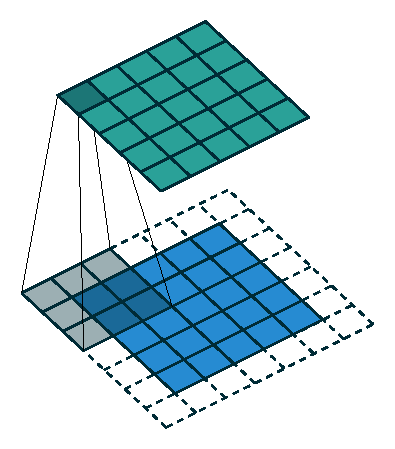
\includegraphics[width=0.23\textwidth]{figures/main/ch2-background/conv_00.pdf}
  \hfill
  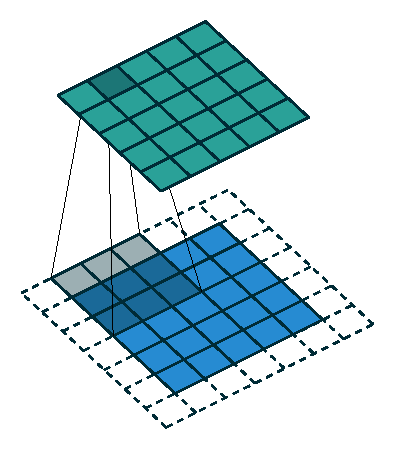
\includegraphics[width=0.23\textwidth]{figures/main/ch2-background/conv_01.pdf}
  \hfill
  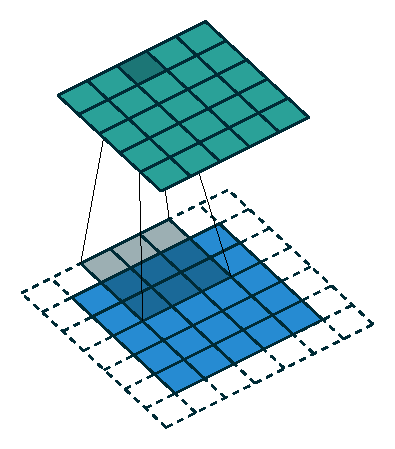
\includegraphics[width=0.23\textwidth]{figures/main/ch2-background/conv_02.pdf}
  \hfill
  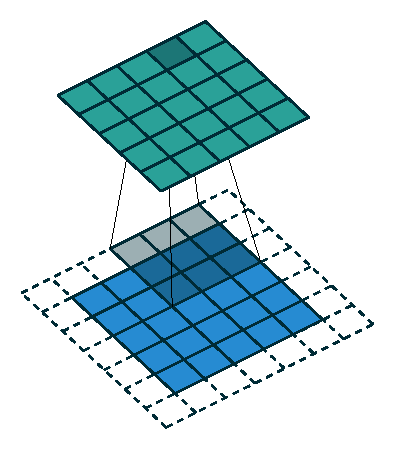
\includegraphics[width=0.23\textwidth]{figures/main/ch2-background/conv_03.pdf}
  \caption{A convolution: a kernel sliding over an image and acting as a filter. \\Illustration taken from~\citet{dumoulin2016guide}.}
  \label{figure:illustration_convolution}
\end{figure}

Doubly-block circulant and doubly-block Toeplitz matrices are very interesting structured due to their relation to 2-dimensional convolutions.
Recall that a discrete convolution can be seen as a kernel sliding over the image and acting as a filter.
\Cref{figure:illustration_convolution} illustrates the convolution operation with the image (blue), the kernel (gray) and the resulting operation (green).
It has been shown by~\citet{jain1989fundamentals} that the convolution operation is a linear transform `performed' by a doubly-block Toeplitz matrix (in the 2d case), \ie, a block Toeplitz matrix where the blocks are also Toeplitz.
Considering convolutions as a simple linear transform with a structured matrix has allowed multiple results to be derived~\citet{appuswamy2016structured,wang2020orthogonal,sedghi2018singular,singla2019bounding}, including one of our main contributions presented in \Cref{chapter:ch5-lipschitz_bound}.



% This observation has been made by~\citet{jain1989fundamentals} and many works have been derived from it~\citet{appuswamy2016structured,wang2020orthogonal,sedghi2018singular,singla2019bounding}, including one of our main contributions presented in \Cref{chapter:ch5-lipschitz_bound}.

A discrete convolution operation with a 2-dimensional kernel applied on a 2-dimensional signal is equivalent to a matrix multiplication with a doubly-block Toeplitz matrix.
Let $\Kmat$ be a 2-dimensional kernel defined as follows:
\begin{equation*}
  \Kmat = \leftmatrix
    k_0 & k_1 & k_2 \\
    k_3 & k_4 & k_5 \\
    k_6 & k_7 & k_8 
  \rightmatrix
\end{equation*}
then, the doubly-block Toeplitz matrix $\Mmat$ that performs the convolution can be represented as:
\begin{equation*}
  \Mmat = \leftmatrix
    \Tmatsf^{(0)} & \Tmatsf^{(1)} &             &  0          \\
    \Tmatsf^{(2)} & \Tmatsf^{(0)} & \ddots      &             \\
                  & \ddots        & \Tmatsf^{(0)} & \Tmatsf^{(1)} \\
    0             &               & \Tmatsf^{(2)} & \Tmatsf^{(0)}
  \rightmatrix
\end{equation*}
where $\Tmatsf^{(j)}$ are Toeplitz matrices and the values of the kernel $\Kmat$ are distributed in the Toeplitz blocks as follows:

\begin{equation*}
  \Tmatsf^{(0)} = \leftmatrix
    k_4 & k_3 &         &         & 0       \\
    k_5 & k_4 & k_3 &         &         \\
            & k_5 & \ddots  & \ddots  &         \\
            &         & \ddots  & k_4 & k_3 \\
    0       &         &         & k_5 & k_4
  \rightmatrix \quad \quad
  \hfill
  \Tmatsf^{(1)} = \leftmatrix
    k_7 & k_6 &         &         & 0       \\
    k_8 & k_7 & k_6 &         &         \\
            & k_8 & \ddots  & \ddots  &         \\
            &         & \ddots  & k_7 & k_6 \\
    0       &         &         & k_8 & k_7 \\
  \rightmatrix \quad
\end{equation*}

\begin{equation*}
  \Tmatsf^{(2)} = \leftmatrix
    k_1 & k_0 &         &         & 0       \\
    k_2 & k_1 & k_0 &         &         \\
            & k_2 & \ddots  & \ddots  &         \\
            &         & \ddots  & k_1 & k_0 \\
    0       &         &         & k_2 & k_1 \\
  \rightmatrix
\end{equation*}


However, in practice, the signal can have multiple channels (\eg, images have 3 channels: RGB).
% corresponding to the colors red, green and blue).
Let us denote by $\cin$ and $\cout$ the number of channels of the input and output respectively.
Then the convolution takes an input of size $\cin \times n \times n$, performed by a kernel of size $\cout \times \cin \times k \times k$, and outputs a signal of size $\cout \times m \times m$ with $m = n - k + 2p + 1$ where $p$ corresponds to the padding.
The matrix for the multi-channel convolution is the concatenation of $\cout \cdot \cin$ doubly-block Toeplitz matrices.





%%%%%%%%%%%%%%%%%%%%%%%%%%%%%%%%%%%%%%%%%%%%%%%%%%%%%%%%%%%%%%%%%%%%%%%%%%%%%%%
\subsection{LDR: General Framework for Structured Matrices}
\label{subsection:ch2-general_frameworks_for_structured_matrices}
%%%%%%%%%%%%%%%%%%%%%%%%%%%%%%%%%%%%%%%%%%%%%%%%%%%%%%%%%%%%%%%%%%%%%%%%%%%%%%%


Other structured matrices can benefit from reduced memory footprint and fast matrix-vector product.
Bellow a description of some known structured matrices: 
\begin{itemize}
  \item \textbf{Hankel matrix}: A Hankel matrix, named after Hermann Hankel, has constant values along each of its anti-diagonals.
  \item \textbf{Vandermonde matrix}: A Vandermonde matrix, named after Alexandre-Théophile Vandermonde, is a matrix where each term follows a geometric progression.
    A very important special case is the complex matrix associated with the Discrete Fourier transform (DFT) presented in \Cref{definition:ch2-fourier_matrix} which has a Vandermonde structure.
  \item \textbf{Cauchy matrix}: A Cauchy matrix, named after Augustin Louis Cauchy, is an $m \times n$ matrix with elements $a_{ij}$ such that $a_{ij} = (\uvec_i - \vvec_j)^{-1}$ with $\uvec_i - \vvec_j \neq 0$, $i \in \{0,\dots,m-1\}$ and $j \in \{0,\dots,n-1\}$.
\end{itemize}
\Cref{figure:ch2-example_structure_matrices} shows the representation of the parameters sharing of Hankel, Vandermonde and Cauchy matrices.
These matrices with matrices from the Toeplitz family can be unified thanks to the notion of \emph{Low Displacement Rank} (LDR).
Although these matrices appear to have very different kinds of parameter sharing, they can be all associated with a specific displacement operator $\triangleopdown_{\Amat, \Bmat}: \Rbb^{m \times n} \rightarrow \Rbb^{m \times n}$ which takes a matrix, $\Mmat$, and outputs a low rank matrix $\triangleopdown_{\Amat, \Bmat}(\Mmat)$ such that $\rank(\triangleopdown_{\Amat, \Bmat}(\Mmat)) \ll \min(m,n)$.


\begin{figure}[t]
   \centering
   \begin{subfigure}[b]{0.32\textwidth}
       \centering
       \begin{equation*}
	  \leftmatrix
	     \hvec_{n-1} & \cdots     & \hvec_1 & \hvec_0      \\
	     \vdots      & \ddots     & \hvec_0 & \hvec_{-1}   \\
	     \hvec_1     & \ddots     & \ddots  & \vdots       \\
	     \hvec_0     & \hvec_{-1} & \cdots  & \hvec_{-n+1} \\
	  \rightmatrix
       \end{equation*}
       \caption*{Hankel}
   \end{subfigure}
   \hfill
   \begin{subfigure}[b]{0.32\textwidth}
       \centering
       \begin{equation*}
	  \leftmatrix
	    1 & \vvec_0     & \cdots & \vvec_0^{n-1} \\
	    1 & \vvec_1     & \cdots & \vvec_1^{n-1} \\
	    1 & \vdots      &        & \vdots        \\
	    1 & \vvec_{n-1} & \cdots & \vvec_{n-1}^{n-1}
	  \rightmatrix
       \end{equation*}
       \caption*{Vandermonde}
   \end{subfigure}
   \hfill
   \begin{subfigure}[b]{0.32\textwidth}
       \centering
       \begin{equation*}
	  \leftmatrix
	  \frac{1}{\uvec_0 - \vvec_{0}}     & \cdots & \frac{1}{\uvec_0 - \vvec_{n-1}} \\
	  \frac{1}{\uvec_1 - \vvec_{0}}     & \cdots & \frac{1}{\uvec_1 - \vvec_{n-1}} \\
	  \vdots                            & \cdots & \vdots                          \\
	  \frac{1}{\uvec_{n-1} - \vvec_{0}} & \cdots & \frac{1}{\uvec_{n-1} - \vvec_{n-1}}
	  \rightmatrix
       \end{equation*}
       \caption*{Cauchy}
   \end{subfigure}
   \caption{Representation of Hankel, Vandermonde and Cauchy matrices}
  \label{figure:ch2-example_structure_matrices}
\end{figure}


This displacement rank approach has been initially proposed by~\citet{kailath1979displacement} and has been further studied by~\citet{kailath1995displacement,pan2001structured}.
More formally, we can define two displacement operators (for simplification, we consider $m = n$):
\begin{definition}[\emph{Sylvester} \& \emph{Stein} displacement operators]
  Let $\Amat, \Bmat \in \Rbb^{n \times n}$, the \emph{Sylvester} displacement operator denoted $\triangleopdown_{\Amat, \Bmat} = \triangleopdown_{\Amat, \Bmat}: \Rbb^{n \times n} \rightarrow \Rbb^{n \times n}$ is defined as follows:
  \begin{equation}
    \triangleopdown_{\Amat, \Bmat} (\Mmat) \triangleq \Amat \Mmat - \Mmat \Bmat
  \end{equation}
  The \emph{Stein} displacement operator denoted $\triangleopup_{\Amat, \Bmat} = \triangleopup_{\Amat, \Bmat}: \Rbb^{n \times n} \rightarrow \Rbb^{n \times n}$ is defined as follows:
  \begin{equation}
    \triangleopup_{\Amat, \Bmat} (\Mmat) \triangleq \Mmat - \Amat \Mmat \Bmat
  \end{equation}
  where $\triangleopdown_{\Amat, \Bmat} = \Amat \triangleopup_{\Amat^{-1}, \Bmat}$ if the operator matrix $\Amat$ is non-singular, and $\triangleopdown_{\Amat, \Bmat} = -\triangleopup_{\Amat, \Bmat^{-1}}$ if the operator matrix $\Bmat$ is non-singular.
\end{definition}



\begin{table}[t]
  \centering
  \begin{tabular}{c|c|c|c}
    \toprule
    \multicolumn{2}{c|}{\textbf{Operator Matrices}} & \textbf{Class of structured} & \textbf{Rank of } \\
    \textbf{A} & \textbf{B} & \textbf{matrices M} & $\triangleopdown_{\Amat, \Bmat}(\Mmat)$ \\
    \midrule
    $\Zmat_1$                & $\Zmat_{-1}$             & Toeplitz               & $\leq 2$ \\
    $\Zmat_1$                & $\Zmat_0^\top$           & Hankel                 & $\leq 2$ \\
    $\Zmat_0 + \Zmat_0^\top$ & $\Zmat_0 + \Zmat_0^\top$ & Toeplitz + Hankel      & $\leq 4$ \\
    $\diag(\vvec)$           & $\Zmat_0$                & Vandermonde            & $\leq 1$ \\
    $\Zmat_0$                & $\diag(\vvec)$           & Inverse of Vandermonde & $\leq 1$ \\
    $\diag(\uvec)$           & $\diag(\vvec)$           & Cauchy                 & $\leq 1$ \\
    $\diag(\vvec)$           & $\diag(\uvec)$           & Inverse of Cauchy      & $\leq 1$ \\
    \bottomrule
  \end{tabular}
  \caption{Displacing Matrices Associated with Families of Structured Matrices.}
  \label{table:ch2-displacing_matrices}
\end{table}



\noindent
Based on this definition, if $\Mmat$ is a structured matrix, there exist operator matrices $\Amat$ and $\Bmat$ such that $\triangleopdown_{\Amat, \Bmat} (\Mmat)$ is low rank.
In particular, $\Amat$ and $\Bmat$ can be chosen to be diagonal or $f$-unit-circulant matrices (see \Cref{definition:ch2-f_circulant_matrix}) for several classes of structured matrices.
\Cref{table:ch2-displacing_matrices} shows some specific choices of operators for the four basic classes of structured matrices and for some related matrices.
We now define the matrices that can be considered structured with respect to the Sylvester or Stein operator.
\begin{definition}[L-like matrices]
  For an $n \times n$ matrix $\Mmat$ and an associated operator $\triangleopdown_{\Amat, \Bmat}$ (or $\triangleopup_{\Amat, \Bmat}$), the value $r = \rank(\triangleopdown_{\Amat, \Bmat}(\Mmat))$ (or $r = \rank(\triangleopup_{\Amat, \Bmat}(\Mmat))$) is called the \emph{displacement rank}.
    If the value of $r$ is small relative to $n$ as $n$ grows large, then we call the matrix $\Mmat$ \emph{L-like} having a structure of type $L$.
    For example, in the case where the operator $\triangleopdown_{\Amat, \Bmat}$ is associated with Toeplitz matrices (\ie, $\Amat = \Zmat_1$ and $\Bmat = \Zmat_{-1}$, see~\Cref{table:ch2-displacing_matrices}), we call the matrix $\Mmat$, \emph{Toeplitz-Like}.
  \label{definition:ch2-l_like_matrices}
\end{definition}

An important result allows us to express structured matrices with low-displacement rank directly as a function of its low displacement generators.
For the Stein type displacement operator, the following result holds:
\begin{theorem}[Krylov Decomposition~\citet{pan2003inversion,sindhwani2015structured}] \label{theorem:ch2-krylov_decomposition}
  If an $n \times n$ matrix $\Mmat$ is such that $\triangleopup_{\Amat, \Bmat}(\Mmat) = \Gmat \Hmat^\top$ where 
  $\Gmat = (\gvec^{(1)} \ldots \gvec^{(r)}), \Hmat = (\hvec^{(1)} \ldots \hvec^{(r)}) \in \Rbb^{n \times r}$ 
  and the operator matrices satisfy: $\Amat^n = a \Imat$, $\Bmat^n = b \Imat$ for some scalars $a, b$, then $\Mmat$ can be expressed as: 
  \begin{equation} \label{equation:ch2-krylov_decomposition}
    \Mmat = \frac{1}{1 - ab} \sum_{j=1}^{r} ~\krylov(\Amat, \gvec^{(j)}) ~\krylov(\Bmat^\top, \hvec^{(j)})^\top
  \end{equation}
  where $\krylov(\Amat, \vvec)$ is defined by:
  \begin{equation}
    \krylov(\Amat, \vvec) = [\vvec~~\Amat\vvec~~\Amat^2 \vvec~~\ldots~~\Amat^{n-1} \vvec]
  \end{equation}
  \removespace
\end{theorem}

\noindent
This theorem can be used to decompose structured matrices and define efficient algorithms for matrix-vector products.
For example, this theorem can be simplified for \emph{Toeplitz-like matrices} as follows:
\begin{theorem}[Toeplitz-like matrix decomposition \citet{pan2001structured}] \label{theorem:ch2-toeplitz_like}
  If an $n \times n$ matrix $\Mmat$ satisfies $\triangleopdown_{\Zmat_1, \Zmat_{-1}}(\Mmat) = \Gmat \Hmat^\top$ $(\Mmat \text{ is Toeplitz-like})$ where $\Gmat = (\gvec ^{(1)} \ldots \gvec^{(r)}), \Hmat = (\hvec^{(1)} \ldots \hvec^{(r)}) \in \Rbb^{n \times r}$, then $\Mmat$ can be written as: 
  \begin{equation} \label{equation:ch2-toeplitz_like_matrix_decomposition}
    \Mmat = \sum_{j=1}^{r} \Zmat_1(\gvec^{(j)}) \Zmat_{-1}(\Jmat_n \hvec^{(j)})
  \end{equation}
  where $\Jmat_n$ is the reflection matrix of size $n \times n$ (reflection of the identity matrix such that $\Jmat^2 = \Imat$) and $\Zmat_1$ and $\Zmat_{-1}$ are $f$-unit-circulant matrices (see \Cref{definition:ch2-f_circulant_matrix}).
\end{theorem}
\noindent
In the next chapter, we will see how this general framework have been used in the context of compact neural networks.


